\section{\ExercisePrefixEmbeddedC Display ansteuern \optional}

\optionaltextbox

In diesem Abschnitt lernst du die Ansteuerung des Displays kennen.
Das Display hat eine Auflösung von 480 * 320 Pixeln.
Zunächst wirst du den Bildschirm in verschiedenen Farben ausfüllen und die dafür benötigte Farbcodierung kennenlernen.
Anschließend wirst du Funktionen implementieren, um auf dem Bildschirm regelmäßige Muster und Texte auszugeben.
Alle in dieser Aufgabe verwendeten Funktionen \textbf{müssen in der Datei \filename{display.c} implementiert werden}. 
Tabelle \ref{tab:displayFunctions} dokumentiert das erwartete Verhalten der zu implementierenden Funktionen.
%
\begin{table}
	\centering
	\caption{Wichtige Funktionen und Variablen für das Display}
	\label{tab:displayFunctions}
	\begin{tabular}{p{7cm}p{7cm}}
        \toprule
		\textbf{Funktionen/Variablen} & \textbf{Beschreibung} \\
        \midrule
        \lstinline|void drawRect(int16_t x, int16_t y, int16_t w, int16_t h, uint16_t color)|
        & Zeichnet die Umrandung eines Rechtecks in der Farbe color mit der Breite w und der Höhe h an die Stelle x,y. \\ \hline
		\lstinline|void fillRect(int x1, int y1, int w, int h, uint16_t fillcolor)|
        & Zeichnet ein ausgefülltes Rechteck in der Farbe fillcolor mit der Breite w und der Höhe h an die Stelle x,y. \\ \hline
		\lstinline|void drawPixel(int16_t x, int16_t y, uint16_t color)|
        & Zeichnet ein Pixel an x,y mit der Farbe color. \\ \hline
		\lstinline|void fillScreen(uint16_t color)| 
        & Füllt den gesamten Bildschirm mit der Farbe color. \\ \hline
		\lstinline|uint16_t color565(uint8_t r, uint8_t g, uint8_t b)|
        & Umwandlung von RGB in HEX 565. \\
        \bottomrule
	\end{tabular}
\end{table}

\subsection{Bildschirm umfärben}
Das Display verwendet eine RGB565-Codierung für Farben (auch als \enquote{High Color} bekannt\footnote{\url{https://en.wikipedia.org/wiki/High_color}}).
Bei der RGB565-Codierung werden 5 Bits für Rot, 6 Bits für Grün und 5 Bits für Blau verwendet (siehe Abbildung \ref{fig:rgb565}).

\begin{figure}[!htb]
    \begin{centering}
        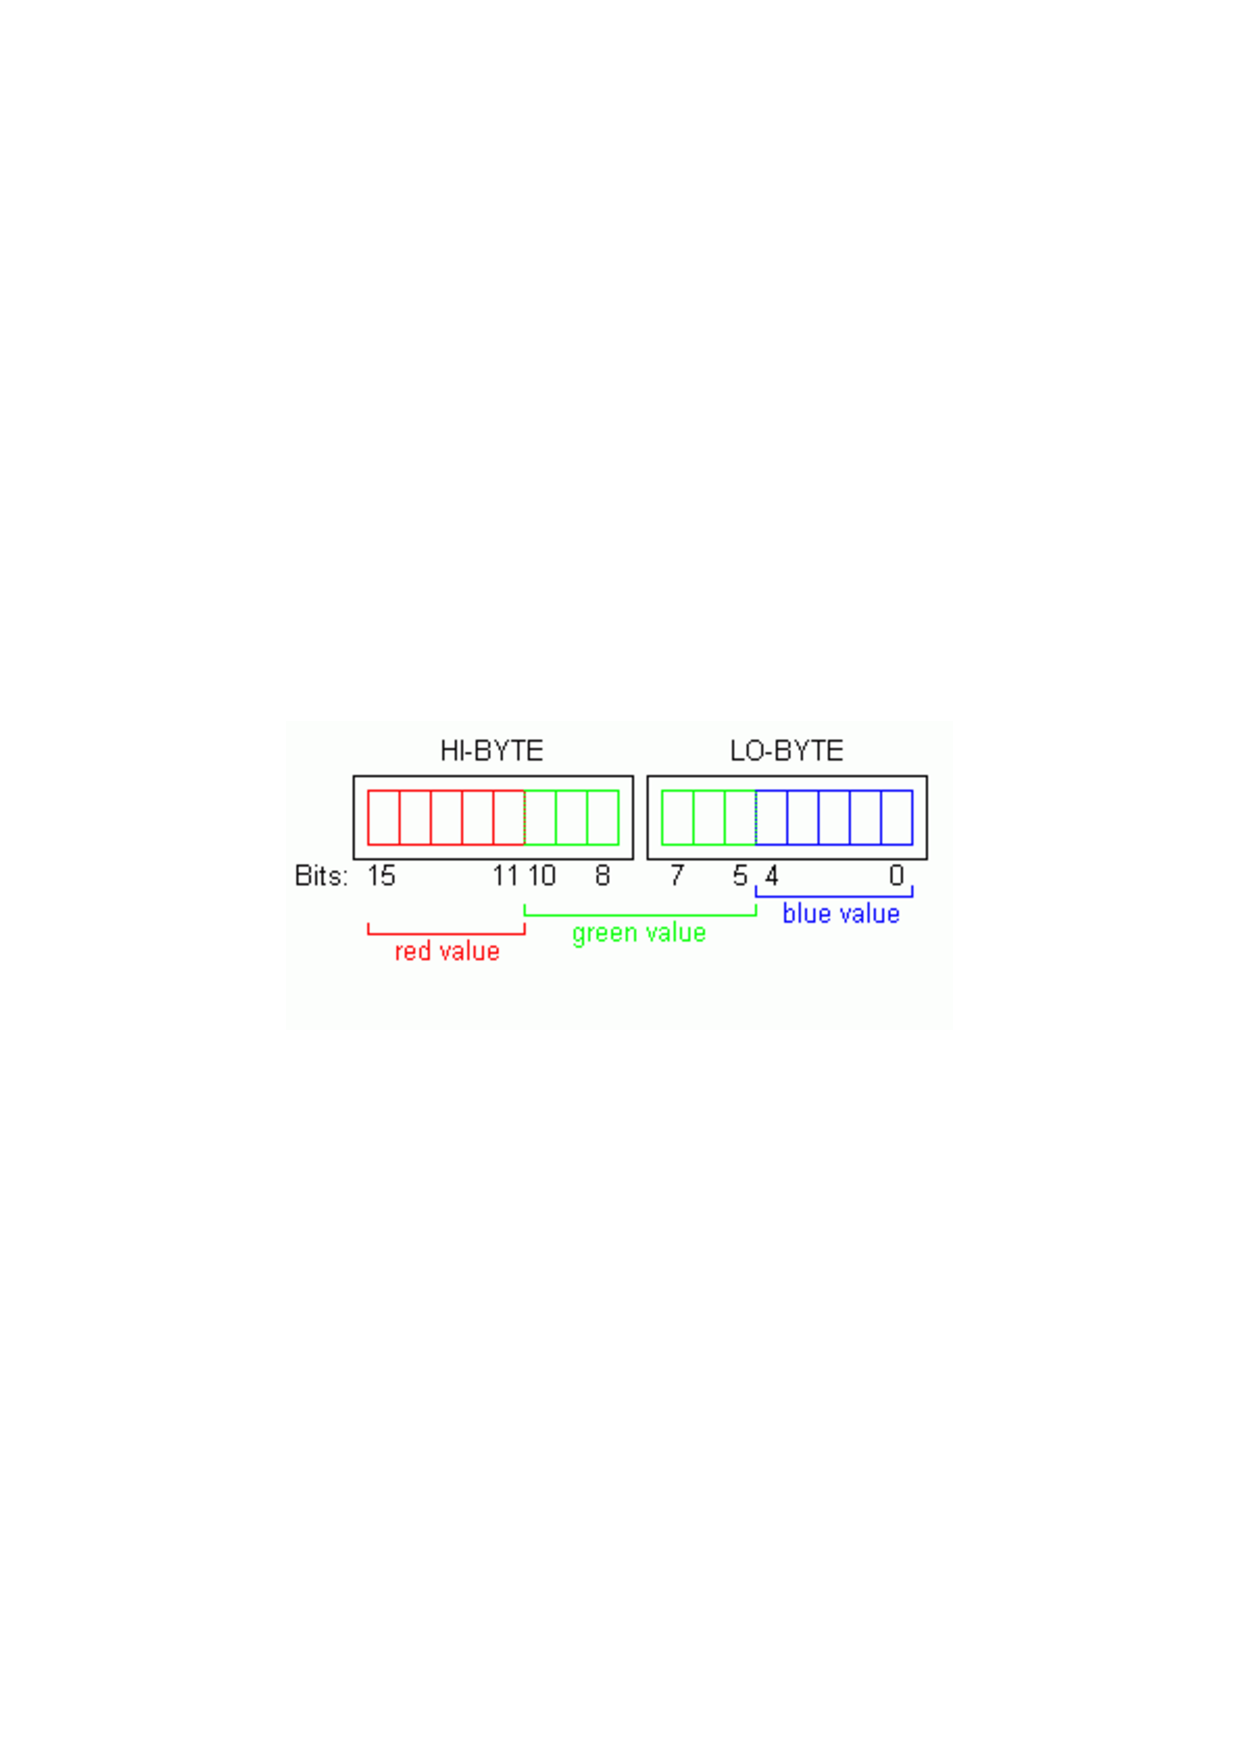
\includegraphics[width=.5\textwidth]{./05_c/figures/rgb565}
        \caption{RGB565 Codierung}
        \label{fig:rgb565}
    \end{centering}
\end{figure}
%
Um auch eigene Farben nutzen zu können, implementierst du zunächst die Funktion \lstinline|color565(uint8_t r, uint8_t g, uint8_t b)|, welche RGB888-Farben in RGB565-Farben umwandelt.
Der Umwandlungsalgorithmus arbeitet für drei gegebene Bytes (\lstinline|uint8_t| oder \lstinline|unsigend char|) \lstinline|r, g, b| wie folgt:
\begin{enumerate}
\item 
Extrahiere die höchstwertigen 5 Bits von \lstinline|r|, die höchstwertigen 6 Bits von \lstinline|g| und die höchstwertigen 5 Bits von \lstinline|b|.
Nutze den Bit-Und-Operator mit einer passenden Bitmaske, um nur die entsprechenden Bits beizubehalten und alle anderen Bits auf 0 zu setzen.
Verwende anschließend den Shift-Operator, um die extrahierten Bits ans untere Ende des Bytes zu schieben.
Es folgt eine Skizze für den Rot-Kanal.

\cpppInputListing{05_c/listings/display_red_channel_example.c}

\item 
Füge die extrahierten Bits mittels des Bit-Oder-Operators zusammen, um den RGB565-Wert zu erhalten:
Beachte dabei, dass du mithilfe des Links-Shift-Operators die einzelnen Teile korrekt ausrichtest.
Beispielsweise muss \lstinline|hiRShifted| vor der Veroderung um 11 Bits nach links verschoben werden.
Beachte, dass das Ergebnis 16 Bit lang sein muss und wir deshalb den Typ \lstinline|uint16_t| verwenden.

\lstinline$uint16_t result=(hiRShifted ____) | (hiGShifted ____ ) | (hiBShifted ____);$
\end{enumerate}

\begin{table}[!htb]
	\centering
	\caption{RGB565-Farbwerte}
	\label{tab:rgb565Table}
	\begin{tabular}{lll}
        \toprule
		\textbf{Farbe} & \textbf{RGB888} & \textbf{RGB565} \\
        \midrule
		Cyan   & \lstinline|0x00EAFF| & \lstinline|0x075F| \\
		Rosa   & \lstinline|0xFC00FF| & \lstinline|0xF81F| \\
		Orange & \lstinline|0xFFB400| & \lstinline|0xFDA0| \\
        \bottomrule
	\end{tabular}
\end{table}

Zum Testen deiner Implementation kannst du die Vergleichswerte in Tabelle \ref{tab:rgb565Table} nutzen.
Gehe dazu wie folgt vor:
\begin{enumerate}
\item 
Lege dir eine leere \lstinline|main|-Funktion an und binde den Header \filename{display.h} ein.
\item 
Füge die folgende Zeile ein, um deinen Code für die Farbe Cyan zu testen:

\lstinline$color565(0x00, 0xEA, 0xFF);$

\item 
Nun erstelle das Projekt wie gewohnt, \emph{aber}, bevor du das Programm auf den Micronctroller lädst, setze einen \emph{Breakpoint} in \lstinline|color565|.
Öffne dazu die Datei \filename{display.c}.
Rechtsklicke in die Zeile, in der die Variable \lstinline|result| zurückgegeben wird.
Wähle \menuPath{Set Breakpoint} (oder drücke \shortcut{F9}).
Links neben der Zeile erscheint ein rotes Rechteck.
\item 
Lade nun den Code auf den Microcontroller.
Die Ausführung sollte an dem eingestellten Breakpoint anhalten (gelber Pfeil).
\item 
Bewege nun den Mauszeiger über die Variable \lstinline|result|.
Es erscheint ein kleiner Tooltip mit dem Inhalt \lstinline|result=1887|.
Dies ist das richtige Ergebnis, aber leider in einer nicht-hexadezimalen Darstellung.
\item 
Um dies zu ändern, öffne die \menuPath{Watch View} mittels \menuPath{View \menuSep Watch} (oder \shortcut{Alt + 3}).
\item 
Betätige die dritte Schaltfläche von links (\enquote{Toggle Hex Mode}) am oberen Rand des \menuPath{Watch}-Fensters.
\item 
Wenn du mit dem Mauszeiger nun erneut auf \lstinline|result| zeigst, erfährst du, dass \lstinline|result=0x075F|.
\item 
Um das Programm weiterlaufen zu lassen, wähle \menuPath{Debug \menuSep Run Control \menuSep Run} (oder \shortcut{F5}).
\end{enumerate}

Die Datei \filename{display.h} enthält einige vordefinierte Farben, die du ebenfalls bei den folgenden Aufgaben nutzen kannst: 
\lstinline|BLACK| (\lstinline|0x0000|), \lstinline|BLUE| (\lstinline|0x001F|), \lstinline|RED| (\lstinline|0xF800|), 
\lstinline|GREEN| (\lstinline|0x07E0|), \lstinline|YELLOW| (\lstinline|0xFFE0|), \lstinline|WHITE| (\lstinline|0xFFFF|).

Im letzten Teil dieser Aufgabe färbst du den Bildschirm mit der Farbe deiner Wahl.
\begin{enumerate}
\item 
Beginne wieder mit einer leeren \lstinline|main|-Funktion.
\item 
Binde die Header \filename{init.h} (aus \winIdeaGroupName{lib}) ein und füge den folgenden Initialisierungscode für das Board in \lstinline|main| ein:

\lstinline|initBoard();|

\item 
Um das Display in Cyan einzufärben, füge folgende Zeile an:

\lstinline|fillScreen(color565(0x00, 0xEA, 0xFF));|
\end{enumerate}


\subsection{Regelmäßiges Muster ausgeben}
In diesem Abschnitt implementierst du die Funktion \lstinline|void printPattern(backgroundColor, foregroundColor)|.
Diese Funktion ordnet auf dem Display Quadrate (4 x 4 Pixel) als Schachbrettmuster an.
%
\hints{
\item 
Nutze die Funktion \lstinline|fillScreen|, um zunächst den Bildschirm in der Farbe \lstinline|backgroundColor| zu füllen.
Nutze anschließend die Funktion \lstinline|fillRect|, um die einzelnen Quadrate in der Farbe \lstinline|foregroundColor| zu erzeugen.
\item 
Eine einfache Möglichkeit ist, zwei geschachtelte \lstinline|for|-Schleifen zu verwenden, die den Schleifenzähler jeweils um die doppelte Blockgröße weiterschalten.
}


\subsection{Text ausgeben}
In diesem Aufgabenteil wirst du einen Cursor implementieren, der es erlaubt, auf einfache Art und Weise Zeichen auf dem Bildschirm auszugeben.
%
\begin{figure}[!htb]
	\begin{centering}
		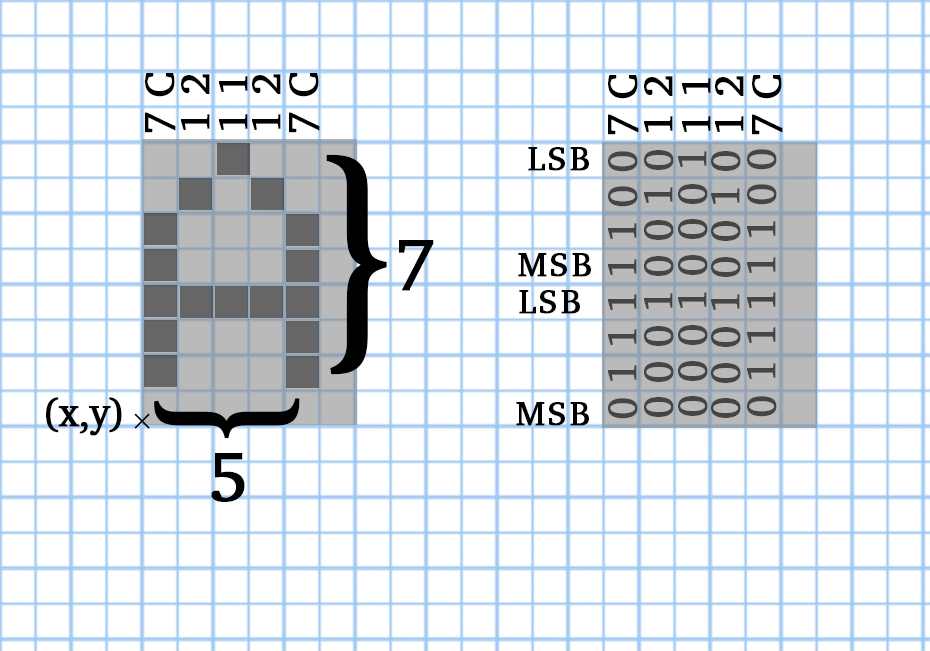
\includegraphics[width=.5\textwidth]{./05_c/figures/ASCII57.png}
		\caption{Schematische Darstellung des Zeichens 'A' in einer ASCII-5*7-Schriftart}
		\label{fig:ascii57}
	\end{centering}
\end{figure}
%
Zum Anzeigen von Buchstaben auf dem Bildschirm stellen wir dir eine kleine Fontbibliothek im Extended-ASCII 5*7-Format zur Verfügung.
Du findest diese in der Datei \filename{glcdfont.h} (Gruppe \winIdeaGroupName{lib}).
Die Bibliothek besteht aus einem Array mit 255 Buchstaben, die jeweils als 5 Bytes abgespeichert sind (siehe Abbildung \ref{fig:ascii57}).
Das 5*7-Format eignet sich für den 480 * 320 großen Bildschirm, da die Darstellung dieser Schriftart mit einer Fläche von 35 Pixeln je Buchstaben immer noch gut lesbar ist.
Wenn man von einem Pixel Abstand zwischen den Buchstaben ausgeht, passen auf das Display bis zu 3200 Zeichen.

Du wirst in dieser Aufgabe mehrere Funktionen in der Datei \filename{display.c} implementieren.
Der Koordinatenursprung $(0,0)$ des Bildschirms ist links unten.
In der Vorlagendatei \filename{display.c} ist die Fontbibliothek \filename{glcdfont.h} bereits eingebunden.
Um globale Grundeinstellungen für die Schriftart festzulegen, wurden bereits die Variablen \lstinline|cursorX|, \lstinline|cursorY|, \lstinline|textColor|, \lstinline|textSize| und \lstinline|textBackground| deklariert. 

\begin{enumerate}
\item 
Implementiere die Setter für den Cursor (\lstinline|setCursor(int16_t x, int16_t y)|), die Textfarbe (\lstinline|setTextColor(uint16_t c)|), die Textgröße (\lstinline|setTextSize(uint8_t s)|) sowie die Hintergrundfarbe (\lstinline|setBackgroundColor(int bg)|).

Zudem sollen in der Funktion \lstinline|initCursor| folgende Grundeinstellungen vorgenommen werden: 
Der Cursor ist im Koordinatenursprung, die Textfarbe ist Weiß, die Hintergrundfarbe ist Schwarz und die Textgröße ist 2.

\item
Die Funktion \lstinline|drawChar(x, y, c, color, bg, size)| soll einen Buchstaben \lstinline|c| in ASCII-Schriftart auf dem Display an der Position \lstinline|x|, \lstinline|y| in der Farbe \lstinline|color| mit der Hintergrundfarbe \lstinline|bg| und in der Größe \lstinline|size| abbilden.
\begin{itemize}
\item 
Zunächst muss überprüft werden, ob die angegebene Position gültig ist.
Sofern die Werte die Grenzen des Bildschirms überschreiten, soll die Funktion \lstinline|drawChar| beendet werden.

\item 
Als nächster Schritt soll auf die richtige Stelle des Arrays \lstinline|font| zugegriffen werden und die gesetzten Bits der Hexadezimalwerte als farbiges Pixel interpretiert werden.
Abbildung \ref{fig:ascii57} zeigt den Aufbau der Daten im Array \lstinline|font| am Beispiel des Buchstabens \lstinline|'A'|.
Ein beliebiger Buchstabe \lstinline|c| ist in \lstinline|font| an der Position \lstinline|c * 5| gespeichert.
Für diesen Buchstaben werden 5 Byte/40 Bits durchiteriert.
Für jedes gesetzte Bit wird an der entsprechenden Stelle ein Pixel (für \lstinline|size == 1|) oder Rechteck (für \lstinline|size > 1|) auf dem Display ausgegeben.
\item 
Zusätzlich soll nach dem Buchstaben ein Leerraum gesetzt werden.
Der Leerraum soll die Breite \lstinline|size| haben.
\end{itemize}

\item 
Um die Textausgabe auf dem Display für Strings zu ermöglichen, müssen weitere Funktionen implementiert werden, die einen automatischen Cursor verwenden.
Dieser Cursor speichert die Position des letzten geschriebenen Buchstabens.
Die Funktion \lstinline|writeAuto(char c)| soll die Aufgabe übernehmen, einen Buchstaben \lstinline|c| auf dem Display mithilfe von \lstinline|drawChar| zu schreiben und die Cursorposition zu verändern.
Hierbei sind Display-Grenzen und Zeilenumbrüche zu beachten.

\item 
Implementiere die Funktion \lstinline|writeText(const char *text)|, welche einen C-String als Parameter erhält und diesen mithilfe von \lstinline|writeAuto| auf das Display schreibt.

\item 
Implementiere abschließend die Funktion \lstinline|writeTextln(const char *text)|, die sich ähnlich wie \lstinline|writeText| verhält, am Ende der Textausgabe jedoch zusätzlich einen Zeilenumbruch einfügt.

\item 
Implementiere zur Ausgabe von Zahlen die Funktionen \lstinline|writeNumberOnDisplay(const uint8_t *value)| und \lstinline|writeNumberOnDisplayRight(const uint8_t *value)|.
Erstere soll die per Pointer übergebene Zahl linksbündig ausgeben, Zweitere soll die Zahl rechtsbündig ausgeben.
Rechtsbündig bedeutet hier, dass die Ausgabe immer diegleiche Breite hat, egal ob der Wert \lstinline|0| oder \lstinline|65535| ist (also: 5 Ziffern).
Verwende die Funktion \lstinline|itoa| (aus \filename{stdlib.h}\footnote{\url{http://www.cplusplus.com/reference/cstdlib/itoa/}}), um den per Zeiger übergebenen Wert in ein \lstinline|char|-Array zu schreiben und anschließend mittels \lstinline|writeText| auf dem Display aus.
\end{enumerate}

\hints {
    \item Falls du Sonderzeichen darstellen möchtest, kannst du dich an folgender Tabelle orientieren: \url{http://www.theasciicode.com.ar/american-standard-code-information-interchange/ascii-codes-table.png}.
    
    Um beispielsweise ein 'ß' auszugeben, definierst du es einfach als \lstinline{char ss = '\\xE1';}
}

